% !TEX program = xelatex

\documentclass[12pt, a4paper]{report}
\usepackage{graphicx, listings, framed, mdframed, float}
\usepackage{appendix, pdfpages, setspace, color, hyperref}
\usepackage{tocloft}                    % This squashes the Table of Contents a bit
\hypersetup{colorlinks=true}            % To avoid the borders around hyperlinks
\hypersetup{colorlinks, citecolor=black, filecolor=black, linkcolor=black, urlcolor=black}
\definecolor{MyLightYellow}{cmyk}{0,0.,0.2,0} % Used for program listings 
\definecolor{shadecolor}{cmyk}{0,0.2,0,0} % Used for snugshade listings 
\usepackage[top=3cm, bottom=3cm]{geometry}% page margins
\setlength{\parskip}{10pt}                % sets spacing between paragraphs
\interfootnotelinepenalty=500             % this prevents footnotes breaking across pages
\renewcommand\bibname{References}         % to change Bibliography to References
\renewcommand\lstlistlistingname{List of Code Listings}
\newcommand{\HRule}{\rule{\linewidth}{0.75mm}} % needed on title page

\begin{document}

\begin{titlepage}   % Standard template for title page. Please don't change layout.
\begin{center}
% Upper part of the page

\includegraphics[width=0.4\textwidth]{BigCrest}\\ \vspace{15 mm}   
\textsc{\Large Year 2 Project}\\ \vspace{15 mm}
\doublespace
\HRule \\ \vspace{8 mm}
{\huge \bfseries Dissertation Writing Guide}       % <<<< Put your title here
\\\vspace{4 mm}
\HRule \\ \vspace{25 mm}
\textbf{Waleed Al-Nuaimy} \\ {\color{MyLightYellow}% <<<< REMOVE THIS LINE <<<<
Name \textsc{Surname1} (ID 2054321)      \\        % <<<< Your names
Name \textsc{Surname2} (ID 2052234)      \\        % <<<< Your names
Group 00                                 \\        % <<<< Your group number

\vspace{15mm}
\emph{Supervised by } Dr Name \textsc{Surname}     % <<<< Your supervisor
}                                                  % <<<< REMOVE THIS LINE <<<<
\vfill             % Bottom of the page
{\large \today}    % today's date
\end{center} \end{center}
\end{titlepage}


\begin{abstract}
This document serves as a template to show you how to present and structure your project dissertation. In the interests of uniformity of format, you are asked not to significantly alter the format and layout of this \LaTeX~ document. The chapter names and structure are intended as a guide, and you are welcome to change these as appropriate. While this is not a definitive guide to dissertation writing, it is intended as a guide to assist in documenting and presenting your project work in an academic and professional manner, and reflects the expectations of those in academia and industry who are likely to read your report. Appended to this guide are some real examples of common mistakes that should be avoided. 

Your Abstract is expected to be between 100 and 250 words in length, and should summarise the problem, outline the approach adopted, and summarise the project findings or results. It's the first (and possibly the only) part to be read, and should provide a snapshot of the whole project in 2 or 3 paragraphs.
\end{abstract}

\newpage

\rule{0mm}{30mm}

\centerline{\textbf{Declaration}}

\fbox{\parbox{0.92\textwidth}{I confirm that I have read and understood the University’s definitions of plagiarism and collusion from the Code of Practice on Assessment. I confirm that I have neither committed plagiarism in the completion of this work nor have I colluded with any other party in the preparation and production of this work. The work presented here is my own and in my own words except where I have clearly indicated and acknowledged that I have quoted or used figures from published or unpublished sources (including the web). I understand the consequences of engaging in plagiarism and collusion as described in the Code of Practice on Assessment (Appendix L).}}



\newpage \tableofcontents
\newpage \listoffigures
\newpage \listoftables 
\newpage \lstlistoflistings        % this is for program listings; if you don't have any, remove this line

\newpage \onehalfspace

%-------------------------------------------------------------------------------------------------------
%-------------------------------------------------------------------------------------------------------
\chapter{Introduction}
%-------------------------------------------------------------------------------------------------------
%-------------------------------------------------------------------------------------------------------

There is more to a good project than the experimental results on the bench. The results may be seen by a couple of people on the day of the bench ispection, but the project report or dissertation remains as documentary evidence of your work, for others to refer to when progressing your work further in the future. This document should be something to take pride in, and if you invest time and effort into producing a well-organised and illustrated dissertation, this will undoubtedly pay off. 

The IET has published a useful guide\footnote{\url{http://www.theiet.org/students/resources/technicalreport.cfm}} to report writing~\cite{ref:IET} in which they establish and explain a number of ``laws of report writing'', quoted below: 

\begin{snugshade}
%\begin{quotation} 
\begin{enumerate} \itemsep -5pt
    \item The reader is the most important person.
    \item Keep the report as short as possible. 
    \item Organise for the convenience of the report user.
    \item All references should be correct in all details. 
    \item The writing should be accurate, concise and unobtrusive. 
    \item Put the right diagram with the right labels in the right place for the reader. 
    \item Summaries give the whole picture, in miniature. 
    \item Reports should be checked for technical errors, typing errors and inconsistency.
    \item The report should look as good as it is. 
    \item The reader is the most important person.
\end{enumerate}
%\end{quotation}
\end{snugshade}

%-------------------------------------------------------------------------------------------------------
\section{\LaTeX}
%-------------------------------------------------------------------------------------------------------

This document provides a \LaTeX template for your report. \LaTeX is a typesetting ``language'' intended for technical reporting, and allows you to produce professional and well-structured documents. \LaTeX~is built around the philosophy that authors need only concentrate on the logical structure of their document, rather than worrying about formatting. By using \LaTeX, you are much less likely to loose marks for poor report formatting, and your technical writing will be of a high presentational standad. There are several free \LaTeX~distributions and editors; on campus you can install MikTex, but to get started I suggest you sign up to use the free online \LaTeX~editor and compiler at \url{http://www.scribtex.com} or \url{http://www.verbosus.com}. Please use \textbf{this document} as a template, adding your content gradually in stages, and compiling at every step to check for errors. 

There are plenty of online tutorials (such as~\cite{ref:Latex1},~\cite{ref:Latex2} and~\cite{ref:Bib1}) to assist you in mastering \LaTeX, as well as some free \LaTeX~editors to help in the editing of the text files. For example, you may wish to install the free offline WYSIWYG\footnote{What You See Is What You Get} \LaTeX~ editor such as LyX (\url{http://www.lyx.org} to simplify and automate the editing. You are encouraged to self-learn this aspect. It is hoped that mastering \LaTeX~will allow you to produce high-quality lab and project reports throughout your studies at Liverpool and beyond.

With large documents such as dissertations, you may wish to work on each chapter separately, as this will make compiling faster and more convenient. \LaTeX allows you to insert one file into another when building the document using this command:

\verb| \include{filename}          % don't include the .tex extension|

Very large documents (that usually include many files) take a very long time to compile, and most users find it convenient to test their last changes by including only the files they have been working on by commenting out the others, as shown below. One option is to hunt down all \verb|\include| commands in the inclusion hierarchy and to comment them out. N.B. The individual files that are included (e.g. \texttt{chapter1.tex}) do \textbf{not} need any formatting commands such as \verb|\documentclass or \usepackage| and may start immediately with something like \verb|\chapter{Introduction}|.

\newpage

\begin{snugshade}
	%\begin{mdframed}[linewidth=0.5pt, backgroundcolor=shadecolor]
	\begin{verbatim}
	
	\documentstyle{...}
	...
	\begin{document}
	
	\include{frontstuff}   % title page, abstract, etc
	\include{chapter1}     % note the .tex extension is omitted
	\include{chapter2}
	%\include{chapter3}     % note chapters 3 onwards commented out
	%\include{chapter4}
	%\include{chapter5}
	%\bibliography{MyRefs.bib}
	%\include{appendix}
	...
	\end{document}
	
	\end{verbatim}
	%\end{mdframed}
\end{snugshade}

%-------------------------------------------------------------------------------------------------------
\section{Report Structure}
%-------------------------------------------------------------------------------------------------------

The purpose of a project report is to document your experimental findings and to communicate their relevance and significance. For this to be effective, it must demonstrate your comprehension of the underlying concepts and principles the project was intending to examine. It is not sufficient to simply record the experimental procedure and results. To facilitate this communication, scientists and engineers have adopted a common format for their technical writing, and project dissertations typically consist of a number of chapters, as laid out in this template document. This communication skill is also essential for the authoring of project dissertations, theses and scientific articles and papers~(further guidance can be sought from such references as~\cite{ref:Bib2},~\cite{ref:Mow},~\cite{ref:Bibby},~\cite{ref:Brune} or~\cite{ref:SIR}).
 
The general agreed structure of a scientific project report is as follows:
\begin{enumerate} \addtolength{\itemsep}{-0.5\baselineskip}
    \item Title page to contain name(s) and date
    \item Abstract
    \item Table of Contents
    \item Table of Figures
    \item Table of Tables
    \item Table of Code Listings
    \item Chapter: Introduction
    \item Chapter: Materials and Methods
    \item Chapter: Results and Analysis
    \item Chapter: Discussion and Conclusions
    \item References
    \item (optional) Appendix
\end{enumerate}

It is expected that your project report will contain at least these four chapters, even if you choose to name them differently. It is likely that you will have further chapters (e.g. Chapter: Theory, Chapter: Design and Implementation), either to present further background theory, previous work in the area, explore further commercial applications of the project or to elaborate more on the design and implementation aspects of your project.  
 
%-------------------------------------------------------------------------------------------------------
\section{Title and Abstract Pages}

This should contain project title, group member names \& IDs, supervisor name Department name and date (follow the first page of this document).

The abstract page contains the Abstract; this summarises the report: its purpose, key findings and conclusions, with or without mention of the procedure, in roughly 100 to 250 words. 

Immediately after the Abstract, you have to write out a statement (declaration) concerning plagiarism and collusion, similar to the one shown at the beginning of this report:

\textbf{``I confirm that I have read and understood the University’s definitions of plagiarism and collusion from the Code of Practice on Assessment. I confirm that I have neither committed plagiarism in the completion of this work nor have I colluded with any other party in the preparation and production of this work.....Code of Practice on Assessment (Appendix L).''}

The Abstract page is generally followed by a Table of Contents (use MS Word to create it automatically).  

%-------------------------------------------------------------------------------------------------------
\section{Introduction and Motivation}
%-------------------------------------------------------------------------------------------------------

Sometimes referred to as the ``rationale'' section, this usually includes a statement of the problem to be investigated, and why is addressing this problem worthwhile or important. This section should also introduce the history and theoretical background of the problem, a brief statement of the general procedure adopted and hint at expected results. This section often includes the \textbf{rationale} for the project, which could be commercial, industrial, scientific or even humanitarian. The Introduction is  also the place to present the theoretical or technical background for the task at hand, presenting existing published work or commercial alternatives  that may be available. This helps prepare the reader to better appreciate and understand what you are attempting to achieve in your project, and why. This is the section where you are most likely to be citing published material, and it is here that you need to be most wary of the dangers of inadvertent \emph{plagiarism}: avoid it all costs. If you are convicted of plagiarism, you will receive a zero for your project, and will very likely fail the lab module. There is no resit opportunity for the project, so failing the module will mean failing the year. Don't let it happen to you!

%-------------------------------------------------------------------------------------------------------
\section{Objectives}
%-------------------------------------------------------------------------------------------------------


Use this section to spell out a set of clear and achievable aims and objectives for the project, so the reader can see what you're trying to achieve, and so that the project can be assessed against these objectives, i.e. how well have they been met? The project \textbf{aim} is the overall purpose of what you're doing, while the the \textbf{objectives} are more specific and measurable in relation to the project requirements, building towards the ultimate aim. 

The objectives are distinct from the individual tasks, and represent components of the project usually in chronological order.  There should be a clear outcome that will benefit someone. For example, ``\textit{Develop a 3-dimensional mathematical model for robotic arm}'' is a suitable \textbf{objective}, whereas ``\textit{carry out calculations and simulation on model}'' is a \textbf{task} rather than an objective. Avoid including such objectives as ``\textit{Learn MATLAB}'' or ``\textit{Improve my understanding of Maxwell's equations}'' as while these may be valid learning outcomes/objectives for you the student, they are not considered valid \textbf{project objectives}. This section helps you to establish the scope and limitations of the project, to maintain the reader's expectations and focus. Unless your objectives are clearly stated, the progress and outcome of your project cannot be accurately assessed. 



%-------------------------------------------------------------------------------------------------------
%-------------------------------------------------------------------------------------------------------
\chapter{Materials and Methods}
%-------------------------------------------------------------------------------------------------------
%-------------------------------------------------------------------------------------------------------

The materials list can be a simple list of all the equipment/apparatus used, in as much detail as possible (eg. mention the make/model of things like signal generators, the values of all components, the exact model of any development boards used etc). If you are using software, the name and version of the software is important. It is advisable to include the data sheets of any equipment or components used in the Appendix, if you think this would help the reader.

The Method/Procedure section describes the experimental process in chronological order (i.e. in the order in which they happened). If you did not follow the documented procedure for any reason, make sure this is mentioned (e.g. ``At step 4 four repetitions were performed instead of three, and the data from the second repetition was ignored. This is due to a circuit fault that was discovered that called the accuracy of these readings into question.'')

If you include any figures, make sure you \textbf{caption} them, with a clear label and number (eg. ``Figure 2.1. Circuit diagram of resonance circuit used (taken from~\cite{ref:Radio})''). It is important that you \textbf{refer to} your figures, otherwise they will be ignored, and you will receive no credit for including them. The same applies to tables. Be sure to mention the source of your figure, if you have copied it from somewhere. 
Captions for figures appear \textbf{beneath} the figure; table captions appear \textbf{above} the table. Using \LaTeX, each figure would have a {\tt label}, such as \verb|\label{OpAmp}| allowing you to then refer to the figure easily by saying ``\verb|as shown in Fig.~\ref{Fig:OpAmp}...|''\footnote{The tilde ($\sim$) character in \LaTeX~is a non-breaking space, i.e. a space that will not break at the end of a line, so the ``Fig.'' will never be separated from the number that follows it. This is equivalent to a \textsf{Ctrl-Shift-Space} in Microsoft Word}, and \LaTeX will automatically insert the correct figure number! Graphs should have both \textbf{axes clearly annotated}, mentioning any \textbf{units} (eg. Volts, Hz). 


\begin{figure}[htbp]     \begin{centering}
    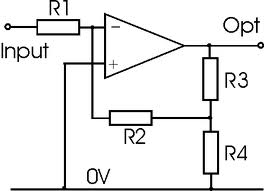
\includegraphics[width=0.5\textwidth]{OpAmp.jpg}
    \caption{Circuit diagram of non-inverting amplifier circuit used in Part 1 (taken from~\cite{ref:Radio})}
    \end{centering}
    \label{Fig:OpAmp}
\end{figure}

%-------------------------------------------------------------------------------------------------------
%-------------------------------------------------------------------------------------------------------
\chapter{Results}
%-------------------------------------------------------------------------------------------------------
%-------------------------------------------------------------------------------------------------------

This is where you describe the important qualitative and quantitative observations from the experiment. Data should be tabulated and/or graphed. Graphs must always be captioned (as with figures, above), and axes clearly annotated with units. Always follow your graphs with a brief description, demonstrating your understanding of what has been plotted (eg. ``The graph in Fig. 4 illustrates the frequency response of this circuit, with a clear resonance peak at 15~kHz.'') as tables and graphs are rarely self-explanatory. If the results differ from what was expected, explain both \textbf{how} (i.e. in what way) and \textbf{why} (i.e. possible reasons behind this behaviour) when referring to these results. 

If you have experimental notes from your log book taken during the experiment, these should be placed in the Appendix, but referred to here (eg. ``Refer to logbook results in the Appendix, page 8.'') This is often the section where you answer any questions that are part of the lab experiment.  Both the question and the answer must be written. This section may also contain an \textbf{Analysis} subsection where the results are subjected to some mathematical or computational analysis, presenting further results to be described here, and discussed more fully in the following section.

The Discussion section allows you to fully discuss and interpret the results and the results of the any analysis carried out. It is also important here to relate your findings to the experimental objectives, i.e. do your results support the theoretical background, and have the objectives of the experiment been met? Are the results reliable and/or significant? 

%-------------------------------------------------------------------------------------------------------
\section{Error Analysis}
%-------------------------------------------------------------------------------------------------------

If your project involves experimental of simulated measurements, it is important that you carry out an analysis of the errors involved, as all measurements contain a degree of uncertainty. You should investigate and detail the different types of error involved, identifying their source, and attempt to quantify each one. If these measurements are used to calculate other quantities, then the \textbf{propagation} of these errors must also be investigated. This will almost certainly involve further reading (that must be referenced correctly), as error analysis needs to be done using sound scientific principles. You should consider ways in which the overall error can be reduced, and report your suggestions in the Discussion chapter.

%-------------------------------------------------------------------------------------------------------
\section{Referencing}
%-------------------------------------------------------------------------------------------------------

If you ever find yourself referring to a previously reported method, book, website, article or even your lab script or lecture notes, you must insert a citation (like this~\cite{ref:BCU}. Every quotation must be referenced. Failure to do this will result in a charge of plagiarism, and is a violation of scientific and literary ethics. There are a number of acceptable formats for listing references, please read up on these separately. You are encouraged to adopt the IEEE referencing style~\cite{ref:IEEE},~\cite{ref:Druker}, provided automatically by the \LaTeX instruction \verb|\bibliographystyle{IEEEtran}|. Please look at the file \verb|MyRefs.bib| and references~\cite{ref:Bib1} and~\cite{ref:Bib2} for guidance on how to correctly format the BibTeX bibliography file for \LaTeX to process correctly. 

Note that it isn't enough simply to include your source in the References section; you need to \textbf{cite} your reference every time you mention something from it (even if you write it in your own words), just as the previous paragraph contains a number of citations between square brackets. Failure to properly cite your sources in this way may also lead to a charge of plagiarism~\cite{ref:cop}. 

When referencing a website, it isn't enough simply mention the URL. You need to include as much information as is available, including the author(s), title, date, organisation and URL, as in the examples below\footnote{Taken from \url{http://www.ittc.ku.edu/~krsna/citing.htm\#Website-Author}}:

\begin{snugshade}
\small
\texttt{First name or initials, Surname. (eds) [if appropriate]  ``Title of page'', (Title of site), [online] date,  URL (Accessed: Access date)}.

P. Hudson,  ``PM, Costello liars: former bank chief'', (The Age), [online] 1998,  \url{http://www.theage.com.au/daily/980916/news/news2.html} (Accessed:  9 February 2000).
\end{snugshade}


%-------------------------------------------------------------------------------------------------------
\section{Writting Style and Formatting}
%-------------------------------------------------------------------------------------------------------

Using \LaTeX will make formatting less of a worry, as it will ensure your report conforms to the adopted format and style, but the guidelines below can be used for guidance in situations where \LaTeX may not be available. There are no hard and fast rules, but reports should generally be written in a standard font (such as Times or Arial) of size 11 point, and be used consistently throughout the report. Margins should be wide enough to allow comments to be written when marked, and the left margin should allow enough space for binding (if appropriate). It is expected that all equations, figures and tables are numbered. When citing references, referring to equations or figures, or mentioning values with units, use a non-breaking space (Ctrl-Shift-Space in MS Word or \verb|~| in \LaTeX) to ensure the two parts are kept together (e.g. \verb|a frequency of 10~kHz|, \verb|as in Figure~\ref{Fig:OpAmp}|).

Keep the use of colour to a minimum, and avoid decorating the pages with unnecessary features such as borders. Try to always write in the third person, and in the passive voice without use of the first person (``I'' or ``we''), e.g. ``The circuit in Figure~\ref{Fig:OpAmp} was connected, and voltage measurements were taken as the frequency was varied.'' Needless to say, it is expected that all pages are numbered, and that the report be free from spelling and grammatical errors, and that capital letters should be used appropriately. All values should appear with the correct units, etc.

To avoid inadvertently over-writing your work, it is good practice to maintain a level of version control by adopting a sensible and consistent file naming convention that includes your surname, the title of the report, and the version number, such as {\tt alnuaimy-report-guide-ver02.pdf}, or {\tt Smith-Exp-17-ver03.pdf}; avoid ambiguous filenames such as {\tt report.pdf}.

\section{Multimedia}

There are times when you may wish to embed some multimedia content into your thesis, such as a webpage, an applet, a video or audio clip, and it is useful in such cases to use QR codes (Quick Response codes) to allow the reader to use a smartphone to get immediate access to the content (most smartphones support QR code scanning, either natively or by means of an third party app). This should be \textbf{in addition} to, rather than instead of the normal way of directing your readers to this content. 

For example, if I wished to direct readers to a couple of YouTube video clips, I could say something like this: ``...as presented in the videos at~\cite{ref:YouTubeReport1} and~\cite{ref:YouTubeReport2}, available via the QR codes in the footnote\footnote{
\includegraphics[width=1.4cm]{QR-MRV.png}\cite{ref:YouTubeReport1}   and   
\includegraphics[width=1.4cm]{QR-anasali.png}\cite{ref:YouTubeReport2}}.'' You can generate QR code images easily using website such as \url{http://goqr.me}, with a resolution of 100$\times$100 pixels, and with a print size of 14mm. 



%-------------------------------------------------------------------------------------------------------
%-------------------------------------------------------------------------------------------------------
\chapter{Discussion and Conclusions}
%-------------------------------------------------------------------------------------------------------
%-------------------------------------------------------------------------------------------------------

%The Conclusions section allows you to fully discuss and interpret the results and the results of the any analysis carried out. It is also important here to relate your findings to the experimental objectives, i.e. do your results support the theoretical background, and have the objectives of the experiment been met? Are the results reliable and/or significant?
%This will involve comparing your obtained results with those expected from the theory. Accounting for any discrepancies is an important aspect of your experimental report, and should also go here. If the difference was a result of experimental error, comment on the nature and source of these errors (human error, systematic error, random error, etc). If the errors resulted from the design of the experiment itself, comment on how the design might be improved. If you feel the lab script itself could be improved, here is the place to make you suggestions.
%In this section, you may also wish to detail any additional work or reading you have done related to this experiment. You may have carried out some simulation or modelling, or may have read a scientific article about the topic, and may wish to discuss this here.

The \textbf{Discussion and Conclusions} chapter is often overlooked when writing a project dissertation, and this could result in you losing valuable marks as it is this chapter that typically distinguishes the ``outstanding'' projects ($>$80\%) from the ``comprehensive'' ($>$60\%). This is your opportunity to impress the reader with the depth and breadth of your understanding, and to demonstrate your awareness of the broader contexts (scientific, industrial, social, economic, etc) into which your projects fits.

\section{So what's the purpose of the Discussion?}

The Discussion has four main functions:
\begin{enumerate}
 \item To \textbf{explain the findings} of your work: these could be experimental results, or the development of a technique, algorithm or product. These findings should be summarised here, even if they were presented in the form of results earlier.

 \item To describe the extent to which these findings support the original \textbf{objectives} stated at the beginning of your dissertation.

 \item \textbf{Self-evaluation} of your work and your achievements: how well did your project go? How could you have done it better? What factors influenced your progress? What are the limitations of your study? How useful is your project to others?

 \item Areas for \textbf{further work}: this could include new areas of investigation you'd like to recommend as a result of your research, or parts of your project which you were unable to complete due to constraints and/or problems encountered.

\end{enumerate}

\section{But I've already presented my results. Why should I ``explain'' them?}

It's important that you assess and comment on your research results, \textbf{explaining} what they actually mean. Comment on any trends, patterns or behaviour, including suggesting explanations for any unexpected results. Compare your results to those expected, both from the theory as well as from other published literature. Do your results represent an improvement over published results? How can this be quantified? Does this improvement come at a cost? Can this cost be quantified and justified?

\section{Is it really a good idea to talk about the \emph{limitations} of my work?}

Absolutely! No study is without it's limitations, and you will have been constrained by many factors such as time, experience, equipment, software or the availability of data. Explaining the ways in which you were constrained and the ways in which the research findings themselves are limited will help the reader appreciate your work better, and will allow a more informed interpretation of the conclusions. %If your study was limited, for example, to 2 dimensions, explaining this limitation is an important part of the Discussion, and will not detract from your work at all.

\section{My supervisor never mentioned any of this. Are you sure it's important?}

Absolutely. Your supervisor will have given you guidance on the technical aspects, leaving you to research and consider the broader aspects. According to the Engineering Council who produce the UK-SPEC~\cite{ref:UK-SPEC}, the UK Standard for Professional Engineering Competence, at BEng level there is an expectation that graduates can demonstrate an awareness of the economic, social, and environmental contexts of their work, including:
\begin{quotation}\noindent
\begin{itemize}
    \item [...] commercial and economic context of engineering processes;
    \item [...] engineering activities to promote sustainable development;
    \item [...] relevant legal requirements governing engineering activities, including personnel, health, safety, and risk (including environmental risk) issues; and
    \item [...] professional and ethical conduct in engineering.
\end{itemize}
\end{quotation}

\subsection{What else can I include to improve my dissertation?}

Again, according to the UK-SPEC~\cite{ref:UK-SPEC}, graduates are expected to demonstrate awareness of the practical application of engineering skills, including
\begin{quotation}\noindent
\begin{itemize}
    \item [...] intellectual property and contractual issues;
    \item [...] appropriate codes of practice and industry standards;
    \item [...] technical uncertainty.
\end{itemize}
\end{quotation}


%---------------------------------------------------------------------------------------------
\section{Applications}
%---------------------------------------------------------------------------------------------

What possible applications could this project have? What different industries would benefit from this work? 
How could life be improved as a result of this work? 

%---------------------------------------------------------------------------------------------
\section{Ethical Considerations}
%---------------------------------------------------------------------------------------------

The wider social, cultural and ethical implications of your work and the related technology should also be explored. 
Does this technology raise any particular ethical issues worthy of note, either in itself or by the way it may be applied,  exploited or misused? For example, if your project was about face recognition, you may want to discuss confidentiality privacy issues in dealing with personal data. If your project was about a website that contained a database, you may want to discuss your responsibilities toward the stakeholders in terms of protecting the data from misuse, sale or exploitation. 
 
However if your project is about carrying out laboratory measurements to verify or investigate the relationship between two physical parameters, it might be that there aren’t any obvious ethical issues that arise. You could consider where such devices are typically used, but if this isn't relevant then you needn't be concerned about this section. 


%---------------------------------------------------------------------------------------------
\section{Commercialisation and Intellectual Property}
%---------------------------------------------------------------------------------------------

It would be expected that you explore possible routes for commercialising your work, protecting the intellectual property developed, or disseminating the results of your work. Sometimes the project involves developing an idea, and this idea itself has some value if it is exploited and commercialised. In such cases, it would be expected that you mention how you think this could be achieved. This might involve refining a particular pattern recognition algorithm or the design of a control system or a mobile antenna. Again, this may not apply to a project that is mainly experimental or involves studying the physics of a particular device or verifying a known relationship, so this section may not always be relevant.


%---------------------------------------------------------------------------------------------
\section{Future Work}
%---------------------------------------------------------------------------------------------

How would you extend your project if you had another few weeks to work on it? If another group of students were to continue this project next year, what would you advise them to work on? What areas are there for further development?

%---------------------------------------------------------------------------------------------
\section{Conclusions}
%---------------------------------------------------------------------------------------------

You may want to end your final chapter with a \textbf{Conclusions} subsection that summarises the Discussion, restating what was achieved and what was learnt, indicating briefly what remains to be done, and possibly also summarising the main strengths and weaknesses of the project. 



%-------------------------------------------- References -----------------------------------------------

\singlespace
\bibliographystyle{IEEEtran}               % References section created automatically
\bibliography{MyRefs}                      % The file MyRefs.bib contains the actual bibliography material
\addcontentsline{toc}{chapter}{References} % to add it to the table of contents


% --------------------------- This is how to declare the Appendices section ----------------------------
\newpage
\appendix
\appendixpage
\addappheadtotoc

%-------------------------------------------------------------------------------------------------------
\chapter{Report Marking Descriptors}
%-------------------------------------------------------------------------------------------------------

The following table shows the report marking descriptors that will be used when marking your report.

\begin{table}[htbp]
	\caption{Report Marking Descriptors}
	\begin{center}
		\scriptsize % \footnotesize % \small
		\begin{tabular}{|c|l|l|}
			\hline
			\parbox{0.2\textwidth}{\textbf{Mark Range}} &
			\parbox{0.4\textwidth}{\textbf{Knowledge and Understanding}} &
			\parbox{0.4\textwidth}{\textbf{Intellectual and Practical Skills}} \\
			\hline
			\parbox{0.2\textwidth}{90-99\%\\Outstanding} &
			\parbox{0.4\textwidth}{\rule{0mm}{6mm} Total coverage of the task set. Exceptional demonstration of knowledge and understanding appropriately grounded in theory and relevant literature. \\} &
			\parbox{0.4\textwidth}{\rule{0mm}{6mm} Extremely creative and imaginative approach. Comprehensive and accurate analysis.  Well-argued conclusions.  Perceptive self-assessment. \\} \\
			\hline
			\parbox{0.2\textwidth}{80-89\%\\Excellent} &
			\parbox{0.4\textwidth}{\rule{0mm}{6mm} As Outstanding but with some minor weaknesses or gaps in knowledge and understanding. \\} &
			\parbox{0.4\textwidth}{\rule{0mm}{6mm} As Outstanding but slightly less imaginative and with some minor gaps in analysis and/or conclusions. \\} \\
			\hline
			\parbox{0.2\textwidth}{70-79\%\\Very Good} &
			\parbox{0.4\textwidth}{\rule{0mm}{6mm} Full coverage of the task set. Generally very good demonstration of knowledge and understanding but with some modest gaps. Good grounding in theory. \\} &
			\parbox{0.4\textwidth}{\rule{0mm}{6mm} Some creative and imaginative features. Very good and generally accurate analysis. Sound conclusions.  Some self-assessment. Demonstrates an understanding of the broader context of the task. \\} \\
			\hline
			\parbox{0.2\textwidth}{60-69\%\\Comprehensive} &
			\parbox{0.4\textwidth}{\rule{0mm}{6mm} As ‘Very Good’ but with more and/or more significant gaps in knowledge and understanding and some significant gaps in grounding. \\} &
			\parbox{0.4\textwidth}{\rule{0mm}{6mm} As ‘Very Good’ but analysis and conclusions contain some minor weaknesses, oversights and/or inaccuracies. \\} \\
			\hline
			\parbox{0.2\textwidth}{50-59\%\\Competent} &
			\parbox{0.4\textwidth}{\rule{0mm}{6mm} Covers most of the task set.  Patchy knowledge and understanding with limited grounding in literature. \\} &
			\parbox{0.4\textwidth}{\rule{0mm}{6mm} Rather limited creative and imaginative features. Patchy analysis containing significant flaws.  Rather limited conclusions.  No self-assessment. \\} \\
			\hline
			\parbox{0.2\textwidth}{40-49\%\\Adequate} &
			\parbox{0.4\textwidth}{\rule{0mm}{6mm} As ‘Competent’ but patchy coverage of the task set and more weaknesses and/or omissions in knowledge and understanding.  Just meets the threshold level. \\} &
			\parbox{0.4\textwidth}{\rule{0mm}{6mm} As ‘Competent’ but probably without much imagination.  Shows barely adequate ability to analyse and draw conclusions.  Just meets the threshold level. \\} \\
			\hline
			\parbox{0.2\textwidth}{35-39\%\\Compensatable fail} &
			\parbox{0.4\textwidth}{\rule{0mm}{6mm} Some parts of the set task likely to have been omitted. Major gaps in knowledge and understanding. Some significant confusion.  Very limited grounding. Falls just short of the threshold level. \\} &
			\parbox{0.4\textwidth}{\rule{0mm}{6mm} No creative or imaginative features.  Analysis and conclusions rather limited. Falls just short of the threshold level. \\} \\
			\hline
			\parbox{0.2\textwidth}{20-34\%\\Deficient} &
			\parbox{0.4\textwidth}{\rule{0mm}{6mm} As ‘Compensatable Fail’ but with major omissions and/or major gaps in knowledge and understanding, and/or incorrect approach towards the experimental task Falls substantially below the threshold level. \\} &
			\parbox{0.4\textwidth}{\rule{0mm}{6mm} As ‘Compensatable Fail’ but analysis and/or conclusions may have been omitted, and practical work is substantially below the threshold level. Demonstrates inability to operate or manipulate equipment. \\} \\
			\hline
			\parbox{0.2\textwidth}{0-20\%\\Extremely weak} &
			\parbox{0.4\textwidth}{\rule{0mm}{6mm} Substantial sections of the task not covered. Knowledge and understanding of the task and the laboratory environment very limited and/or largely incorrect.  No grounding in theory. \\} &
			\parbox{0.4\textwidth}{\rule{0mm}{6mm} No creative or imaginative features. No report as such, just collection of notes and/or plots. Analysis extremely weak or omitted. No conclusions. \\} \\
			\hline
		\end{tabular}
	\end{center}
\end{table}






%-------------------------------------------------------------------------------------------------------
\chapter{Examples of Common Elements in \LaTeX}
%-------------------------------------------------------------------------------------------------------

Your appendices may typically include such elements as raw data, data sheets, source code (program listings), photographs, calculations, graphs, pictures or tables that have not been included in the report itself. Sometimes this may involve embedding these as images within the main document. Make sure you refer to each appendix at least once in your report, otherwise they will be ignored.

%------------------------------------------------------------------------------------------------------- 
\section{Tables}
%------------------------------------------------------------------------------------------------------- 

This section contains some table templates to help you create your own tables using \LaTeX. Look at this {\tt .tex} file to see how the table elements are constructed, and use it as a template for your own tables. 

The summary of the experimental results is presented in Table~\ref{tab:summary}

\begin{table}[htbp]
\caption{Note that table captions are placed above the tables, not below as for figures}
\label{tab:summary}
\begin{center}
\begin{tabular}{ccc}
\hline
 $P$ (W)      & $V$ (V)       & $I$ (A)   \\
\hline
$0.0\pm0.01$ & $0.0\pm0.01$ & $0.0\pm0.01$  \\
 0.1         & 0.2          &  0.3         \\
 0.1         & 0.2          &  0.3         \\
 0.1         & 0.2          &  0.3         \\
 0.1         & 0.2          &  0.3         \\
 0.1         & 0.2          &  0.3         \\
 0.1         & 0.2          &  0.3         \\
 0.1         & 0.2          &  0.3         \\
\hline
\end{tabular}
\end{center}
\end{table}


\begin{table}[htbp]
\caption{Resistance and Temperature of the Filament}
\label{tab:data}
\begin{center}
\begin{tabular}{|c||c|c|c|}
\hline
$R$ ($\Omega$) & $T$ (K) & $1/T$ (K$^{-1}$) & $\ln P$ \\
\hline\hline
151.00$\pm$3.92 & 828.35$\pm$23.46& $1.2072\times10^{-3}$& -13.29 \\ \hline
157.12$\pm$3.71 & 856.88$\pm$22.25& $1.1671\times10^{-3}$& -12.64 \\ \hline
162.53$\pm$3.49 & 881.99$\pm$21.02& $1.1338\times10^{-3}$& -12.33 \\ \hline
166.67$\pm$3.33 & 901.14$\pm$20.13& $1.1097\times10^{-3}$& -11.90 \\ \hline
171.84$\pm$3.17 & 924.98$\pm$19.25& $1.0811\times10^{-3}$& -11.25 \\ \hline
176.84$\pm$3.04 & 947.96$\pm$18.53& $1.0549\times10^{-3}$& -10.77 \\ \hline
181.46$\pm$2.90 & 969.13$\pm$15.49& $1.0319\times10^{-3}$& -10.20 \\ \hline
157.12$\pm$3.71 & 856.88$\pm$22.25& $1.1671\times10^{-3}$& -12.64 \\ \hline
162.53$\pm$3.49 & 881.99$\pm$21.02& $1.1338\times10^{-3}$& -12.33 \\ \hline
166.67$\pm$3.33 & 901.14$\pm$20.13& $1.1097\times10^{-3}$& -11.90 \\ \hline
\hline
\end{tabular}
\end{center}  
\end{table}

%-------------------------------------------------------------------------------------------------------
\section{Maths}
%-------------------------------------------------------------------------------------------------------
Mathematical expressions can be included in \LaTeX documents easily by surrounding them in \verb|$| signs, such as $f$, $\delta x$, $\Omega_2$, $y=mx+b$ or $\mu = \frac{1}{N}\sum_{i=1}^N x_i$. Numbered equations can be created just as easily using the \verb|equation| environment: 

\begin{equation}
\mu = \frac{1}{N}\sum_{i=1}^N x_i.
\label{eq:mean}
\end{equation}

When making reference to the above equation, you simply need to mention the label, as in ``\verb|...as shown in Equation~\ref{eq:mean}.|'', and the Equation number will be inserted automatically. If you need to show several lines of mathematical expressions, you can use the \verb|eqnarray| environment as below:

\begin{eqnarray}
  P & = & I V             \\
    & = & I^2 R           \\
    & = & \frac{V^2}{R}
\label{eq:power}
\end{eqnarray}
Further guidance on writing and manipulating mathematical expressions, symbols and equations can be found online in references such as~\cite{ref:Maths}.

%-------------------------------------------------------------------------------------------------------
\section{Program Listings}
%-------------------------------------------------------------------------------------------------------

Program listings and source code can be neatly incorporated into your reports by including them in a \verb|\lstlisting| environment, as in Listing~\ref{myCircleCode} below, or if you are constantly editing your program, you could import the code directly from the source itself (provided you've uploaded it to your ScribTeX workspace). In this way, whenever you modify the source, all you need to do is recompile the \LaTeX code and your report document will automatically be updated. The command to use would be something like \verb|\lstinputlisting{MY_CIRCLE.m}|.

Your code should contain enough comments so that it is readable and understandable. 

\textbf{IMPORTANT NOTE: DO NOT PUT THE CODE AS A SCREENSHOT. THE CODE SHOULD BE PUT IN PLAIN TEXT IN THE REPORT.}

%-------------------------- Source code / program listings can be inserted using like this -----------
\lstset{language=MATLAB, frame=single, basicstyle=\footnotesize, backgroundcolor=\color{MyLightYellow}, breaklines=true,label=myCircleCode}
\begin{lstlisting}[float, caption={Some MATLAB code to draw a circle}]
[x,y] = MY_CIRLCLE(x_centre, y_centre, radius)

% MY_CIRCLE.m - A MATLAB function to draw a circle on the screen
% Syntax is: 
%            [x,y] = MY_CIRLCLE(x_centre, y_centre, radius)
%
% Waleed Al-Nuaimy, 1st July 2011

theta = linspace(0, 2*pi, 200);        % in radians
x     = x_centre + radius*cos(theta);  % radius can be negative!
y     = y_centre + radius*sin(theta);
plot(x,y,'r-')                         % connect using red line 
axis('equal')                          % to preserve aspect ratio
ylabel('y')
xlabel('x')
title(['Circle centred at (',num2str(x_centre),',', ...
       num2str(y_centre),') of radius ',num2str(radius)])
\end{lstlisting}
%-------------------------------------------------------------------------------------------------------

% If you want to link directly to the source code, you'll need to first upload it to this folder, 
% then the command is:  \lstinputlisting[language=MATLAB]{MY_CIRCLE.m}

%-------------------------- Source code / program listings can be inserted using like this -----------
\lstset{language=MATLAB, frame=single, basicstyle=\footnotesize, backgroundcolor=\color{MyLightYellow}, breaklines=true,label=myAreaCode}
\begin{lstlisting}[float, caption={C++ code snippet to calculate area of a circle}]
#include <iostream.h>
#include <math.h> 
int main()
{
double radius;
                                    // user input
cout << "Enter radius : ";
cin  >> radius;
                                    // calculate area
if(radius < 0)
    cout << "Radius must be positive." << endl;
else
    cout << "Area of circle is " << 3.142*pow(radius,2) << endl;

return 0;
}

\end{lstlisting}
%-------------------------------------------------------------------------------------------------------



%-------------------------------------------------------------------------------------------------------
\chapter{Examples of how NOT to write a report}
%-------------------------------------------------------------------------------------------------------

These are some common mistakes, copied from real student reports; try to avoid them!

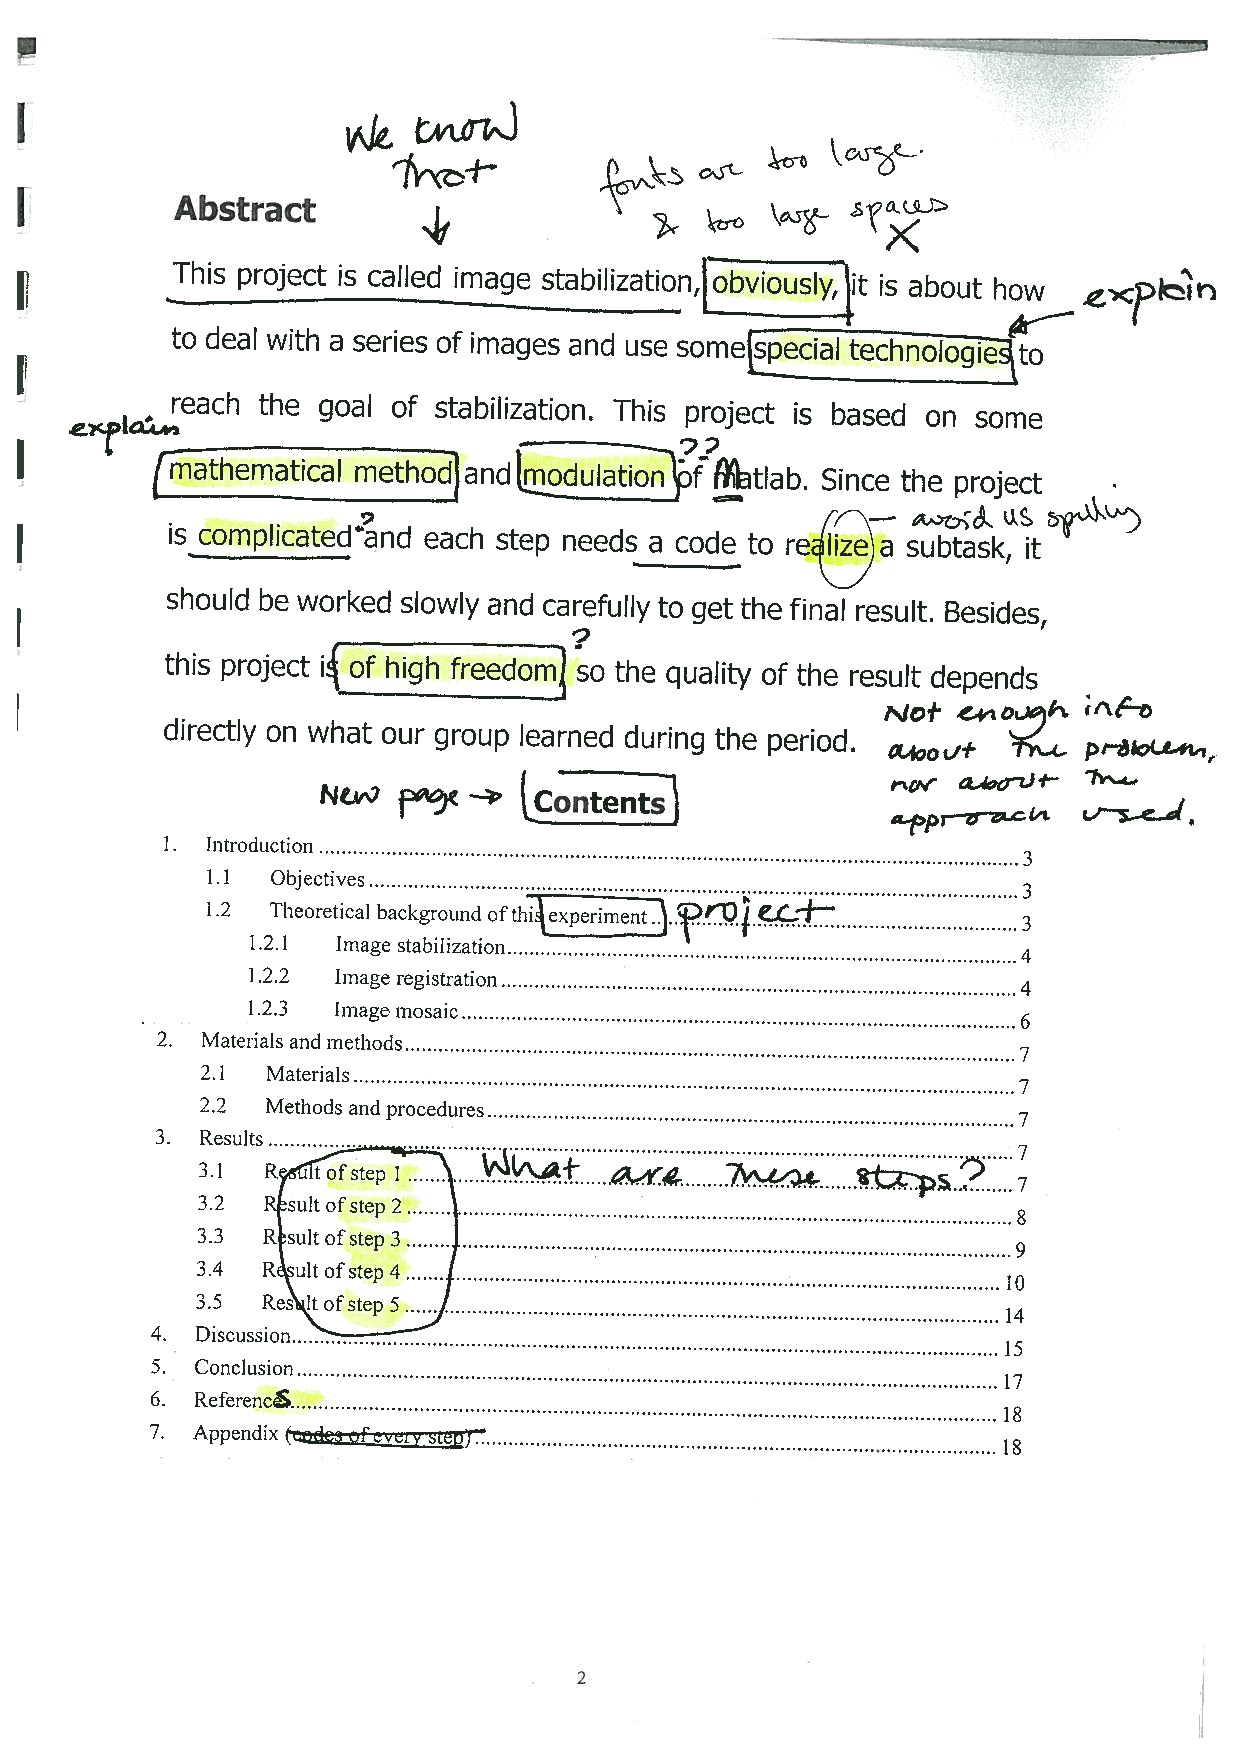
\includepdf[pages=1-]{HowNot.pdf}

\end{document}